\documentclass[../main.tex]{subfiles}

\begin{document}
\section{UCB-BAR: Rocket Chip Generator}
\begin{figure}
    \centering
    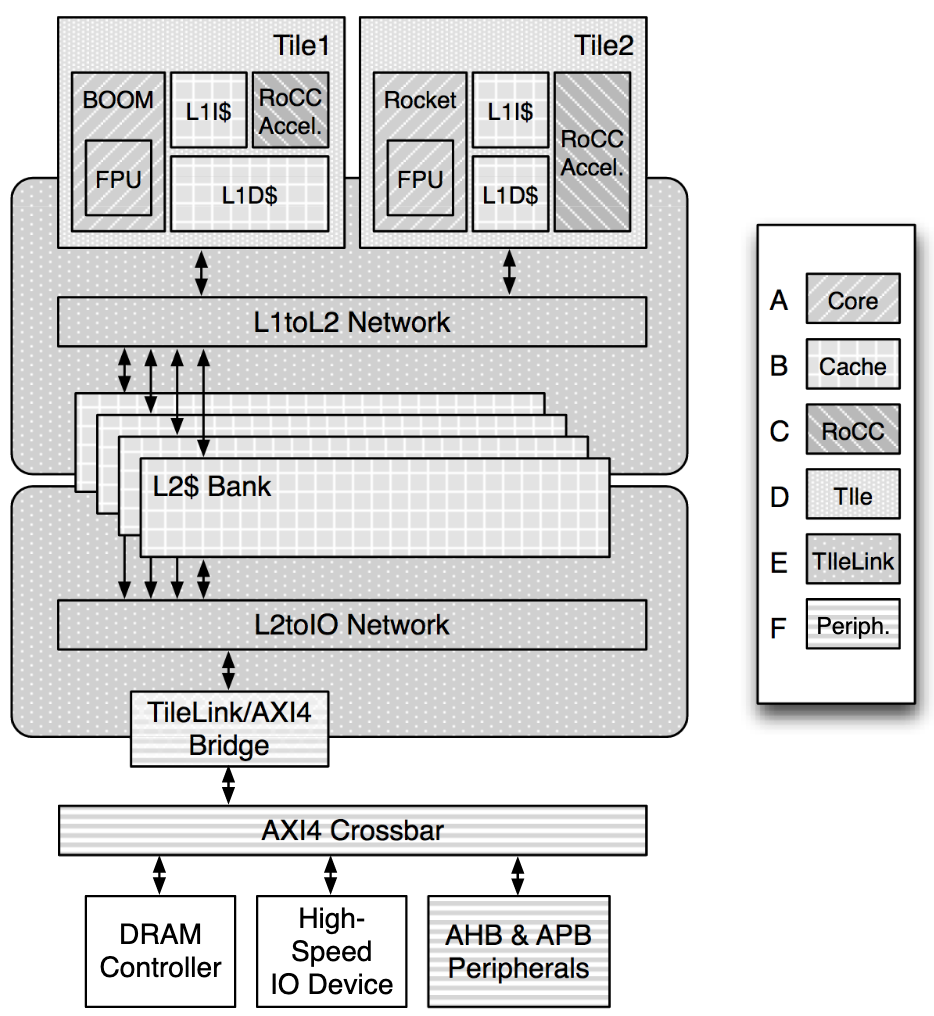
\includegraphics[scale=.5]{pngs/RocketChipGeneratorLayout.png}
    \caption{Rocket Chkp Pipeline\cite{Asanović:EECS-2016-17}}
    \label{fig:RocketCipGen}
\end{figure}
The University of California, Berkeley (UCB) developed the Rocket chip Generator. The Chips Alliance group maintains the generator. This generator produces a system on chip (SOC) with caches and processor tiles. See Figure \ref{fig:RocketCipGen}  for a high-level overview of the SOC generated by the Rocket Chip Generator\cite{Chips-Alliance}.

\subsection{Generic Rocket Chip}
The following is an overview of the SOC generated by the Rocket Chip Generator. At the lowest level is the tiles layer, top of figure \ref{fig:RocketCipGen}, a Tile contains a RISC-V processor L1 data cache, L1 instruction cache. A Tile can have an additional rocket custom co-processor (RoCC). One of UCB most notable RoCC is the Hwacha Vector-Fetch co-processor\cite{HwachaPaper}. Each Tile can instantiate different types of cores: UCB in-order core, Rocket Core, Berkeley out of order machine, BOOM core, or any other custom core. The CHIPS architecture uses the Rocket core in its base design. In the Rocket core, the L1 instruction cache and the L1 data cache are configurable. Each of the tiles connects through a tile link (TL) bus, L1ToL2 network. This network connects the tiles and the L2 caches. Final, the L2 caches connect chip's IO through another TL bus, TLToIO network.


\subsection{Rocket Core}
\begin{figure}
    \centering
    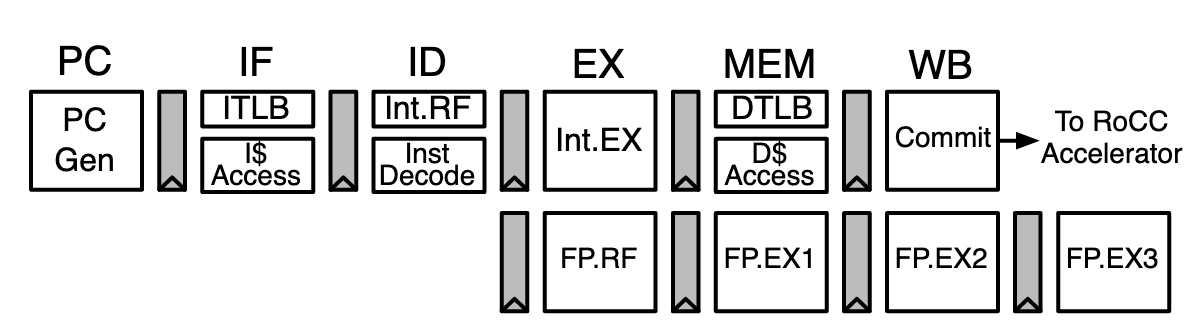
\includegraphics[scale=.4]{pngs/RocketPipeline.png}
    \caption{Rocket Chkp Pipeline\cite{Asanović:EECS-2016-17}}
    \label{fig:RocketCipFlow}
\end{figure}
The Rocket core is a RISC-V based processor. The fundamental core is a single fetch, single issue, in-order scalar processor, see figure \ref{fig:RocketCipFlow}. The fundamental core implements a subset of the RISC-V standard. The following is a list of the supported extensions: integer (I), multiply and divide (M), atomic (A), single-precision (F), and double-precision (D) floating-point. This group of extensions is known as (IMAFG) or (G)\cite{Asanović:EECS-2016-17}. In addition to the S extension group, the Rocket core supports the E extension set. This set is used to communicate with the RoCC unit.  % FIXME need to find ref for E extension


\subsection{Chisel}
The Rocket Chip Generator uses the Chisel domain-specific language (DSL). This DSL uses the Scala programming language as a starting point. Scala provides the ability to use high-level program constructs, and these constructs provide the ability to generate intricate hardware designs. One of the more noteworthy features of Chisel is the ability to extend or reduce the amount of singles in a port list. One of the downside to Chisel is that each set of operators get broken down into sub operators. For example, g = a+b*c gets converted into temp = b*c, g= a + temp. This convention makes the outputted RTL hard to read, so the debugging must be done at the DSL level and not at the RTL level.   

\subsection{Configuring the Rocket Chip Generator}
The Rocket Chip generator works off a set of configuration. Most modules get passed a configuration that determines the functionality of that module. Figure \ref{fig:configsnipit} shows how to add the RoCC co-processor to a default Rocket core on a tile.
%The Rocket Chip Generator uses a set of configures to generator the Rocker Chip in verilog. Each module in the Rocket Chip Generator take a set of configuration. Depending on which set of configuration are set some module will be left out. For example, to have a accelerator added in a tile, extend the base configure and add the configuration for the accelerator. The main configuration file is located in the following directory: /src/main/scale/system/Config.scala. Figure \ref{fig:configsnipit} show an example of such a configuration.
\begin{figure}
    \centering
    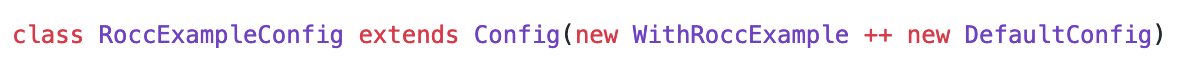
\includegraphics[scale=.4]{pngs/ConfigSnipit.png}
    \caption{ROCC Example Config}
    \label{fig:configsnipit}
\end{figure}
\end{document}